\section{Results}
\subsection{The cosine wave}
The results from the Leapfrog scheme and the Upwind scheme, for the different Courant numbers, can be seen in \autoref{fig:cosine}. There, one can observe that a Courant number of $\mu=1.0$ gave an identical result to the analytical solution, while a Courant number of $\mu=1.1$ made both schemes become unstable. A Courant number of $0.9$ gave slightly damped peaks for the Upwind scheme, while the Leapfrog scheme showed no noticeable deviation from the analytical solution at this timescale.

\begin{figure}[H]
    \centering
    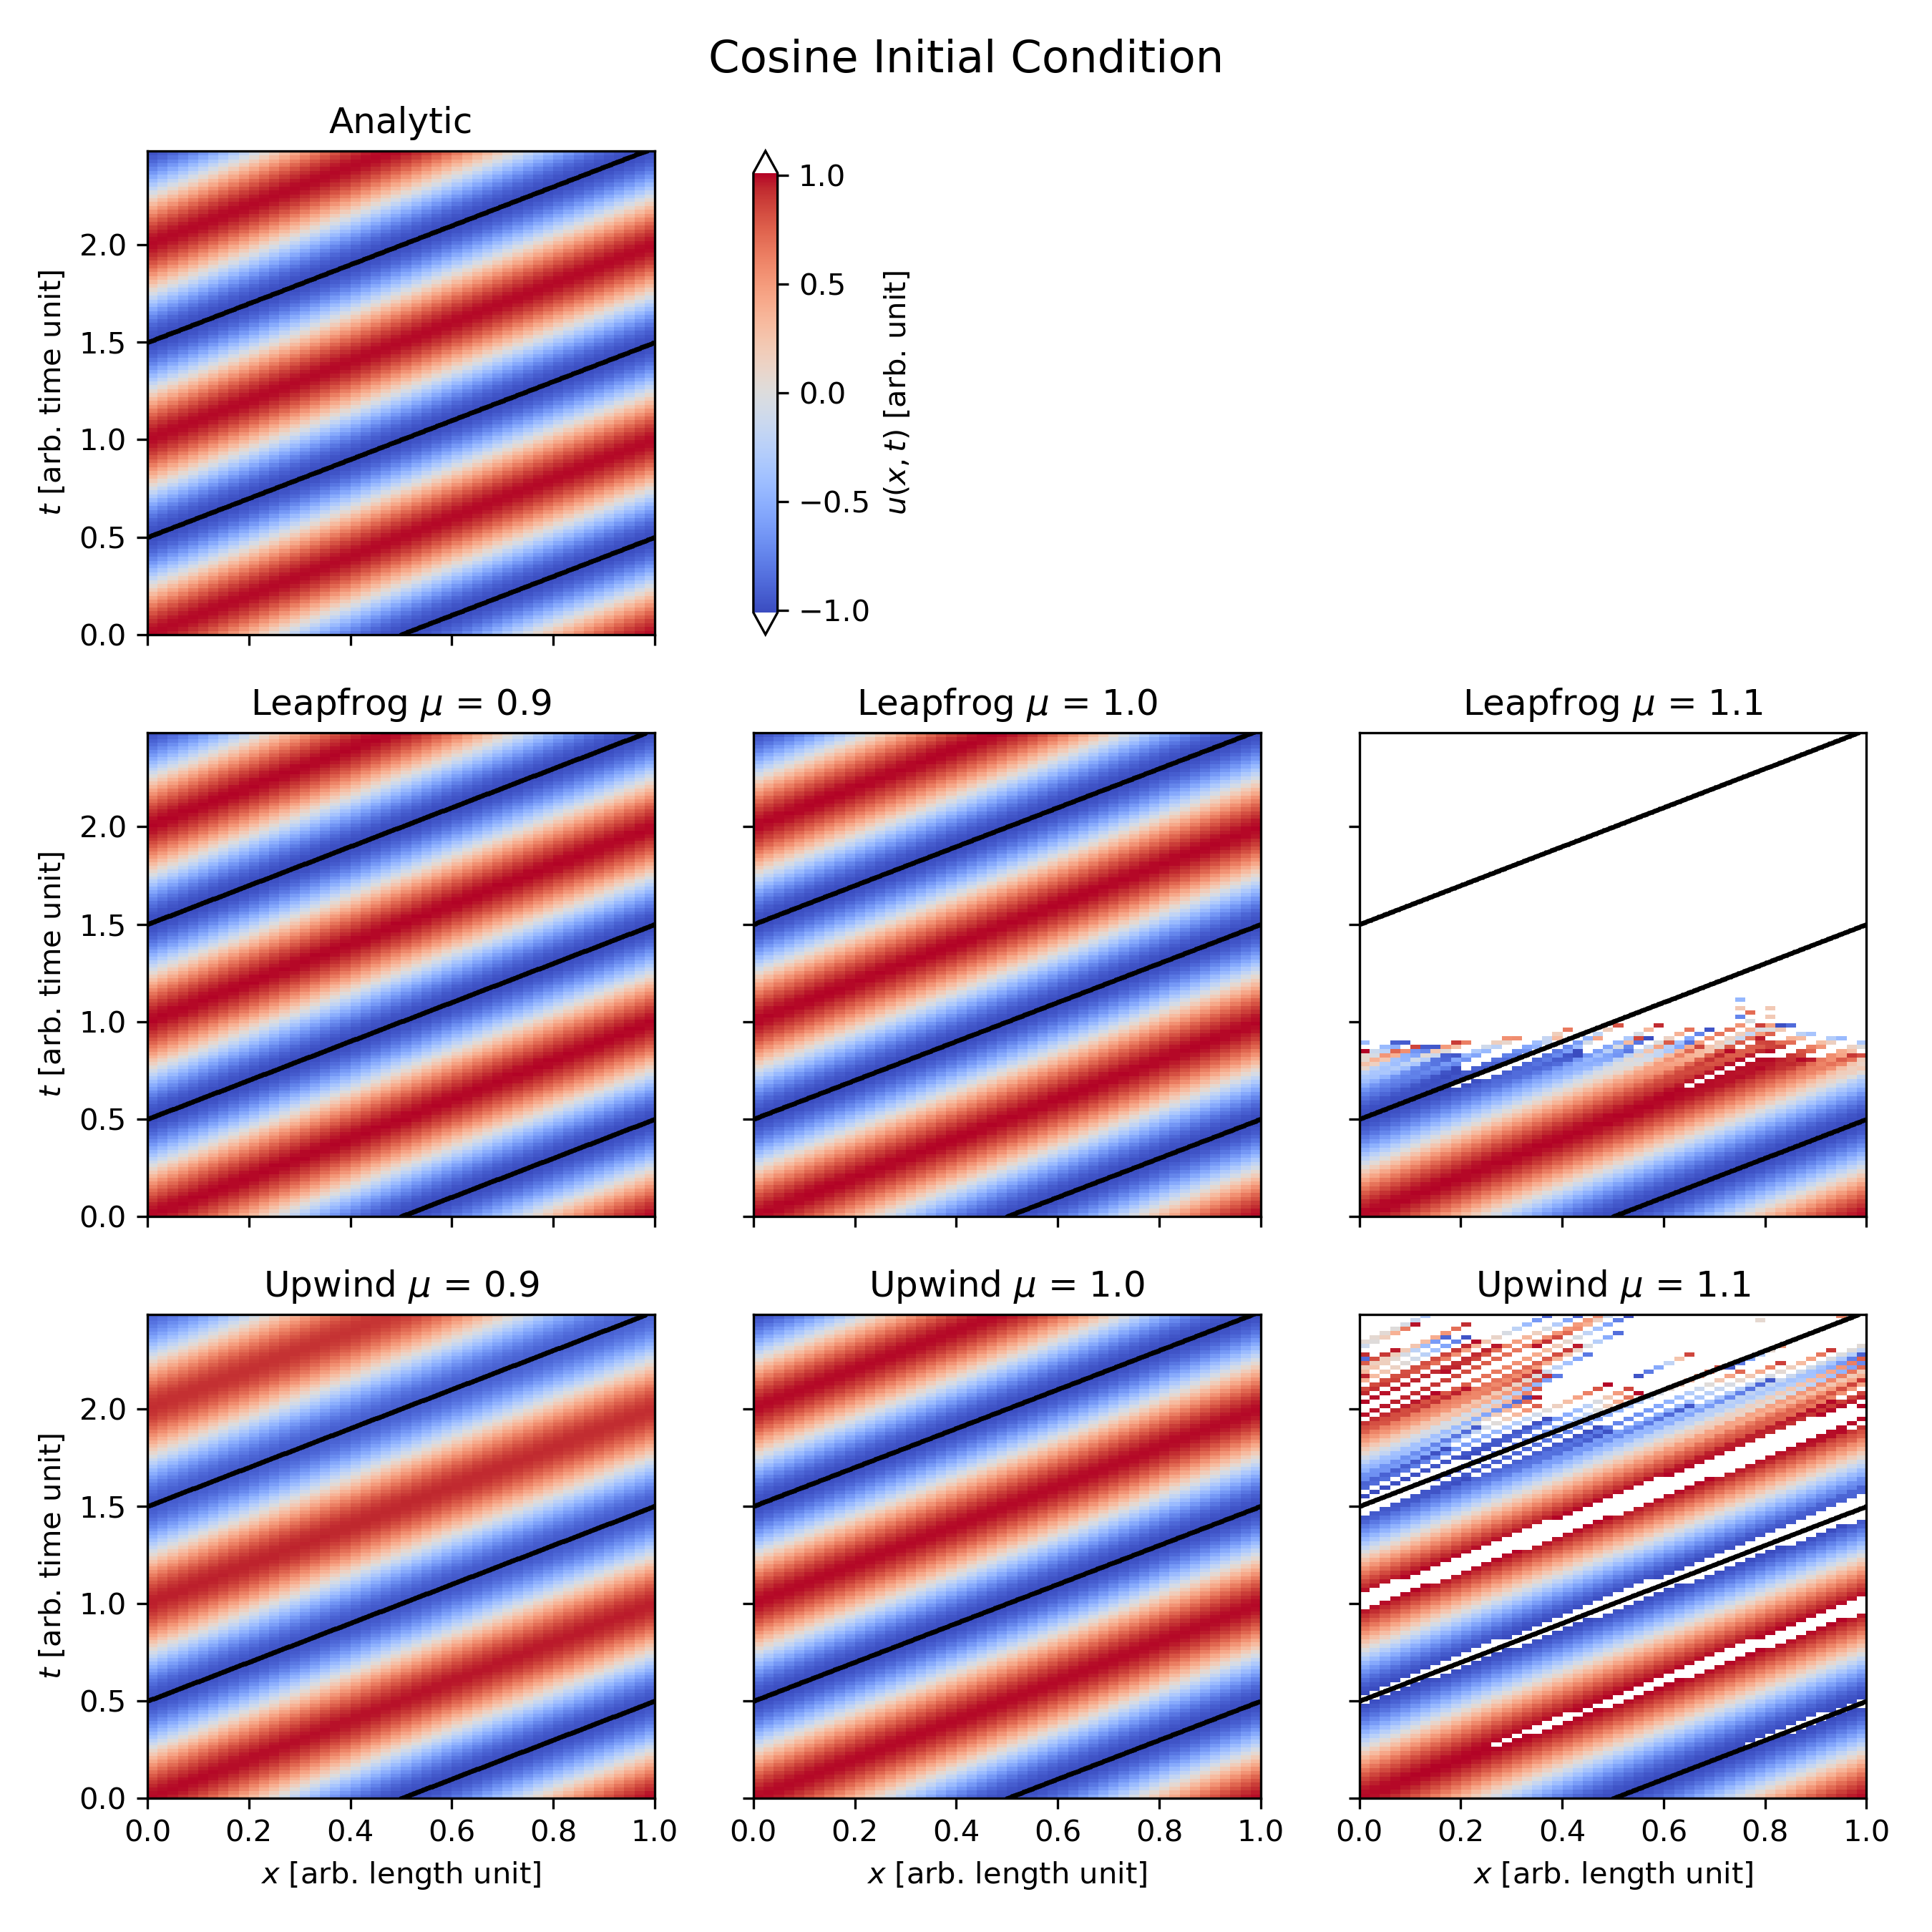
\includegraphics[width=0.85\textwidth]{Figures/cosine-hovmoller.png}
    \caption{This figure shows the solution for the leapfrog scheme, the upwind scheme, along with the analytical solution for various Courant numbers. The black line shows the propagation speed of the analytic solution. Values above or below the analytical values are left as blanc.}
    \label{fig:cosine}
\end{figure}

In \autoref{fig:phaseerrors}, one can observe the phase and amplitude errors from the Leapfrog scheme and Upwind scheme. In both schemes, it can be seen that the numerical schemes are slightly slower than the analytical one. Comparing this value with the theoretical value in \autoref{eq:phasespeed}, one obtains $c_D/c \approx 0.9995$, which is in agreement with the observed phase shift in \autoref{fig:phaseerrors}. Interestingly, a large amplitude drop can be seen in the Upwind scheme, while this is not observed in the Leapfrog scheme.

\begin{figure}[H]
    \centering
    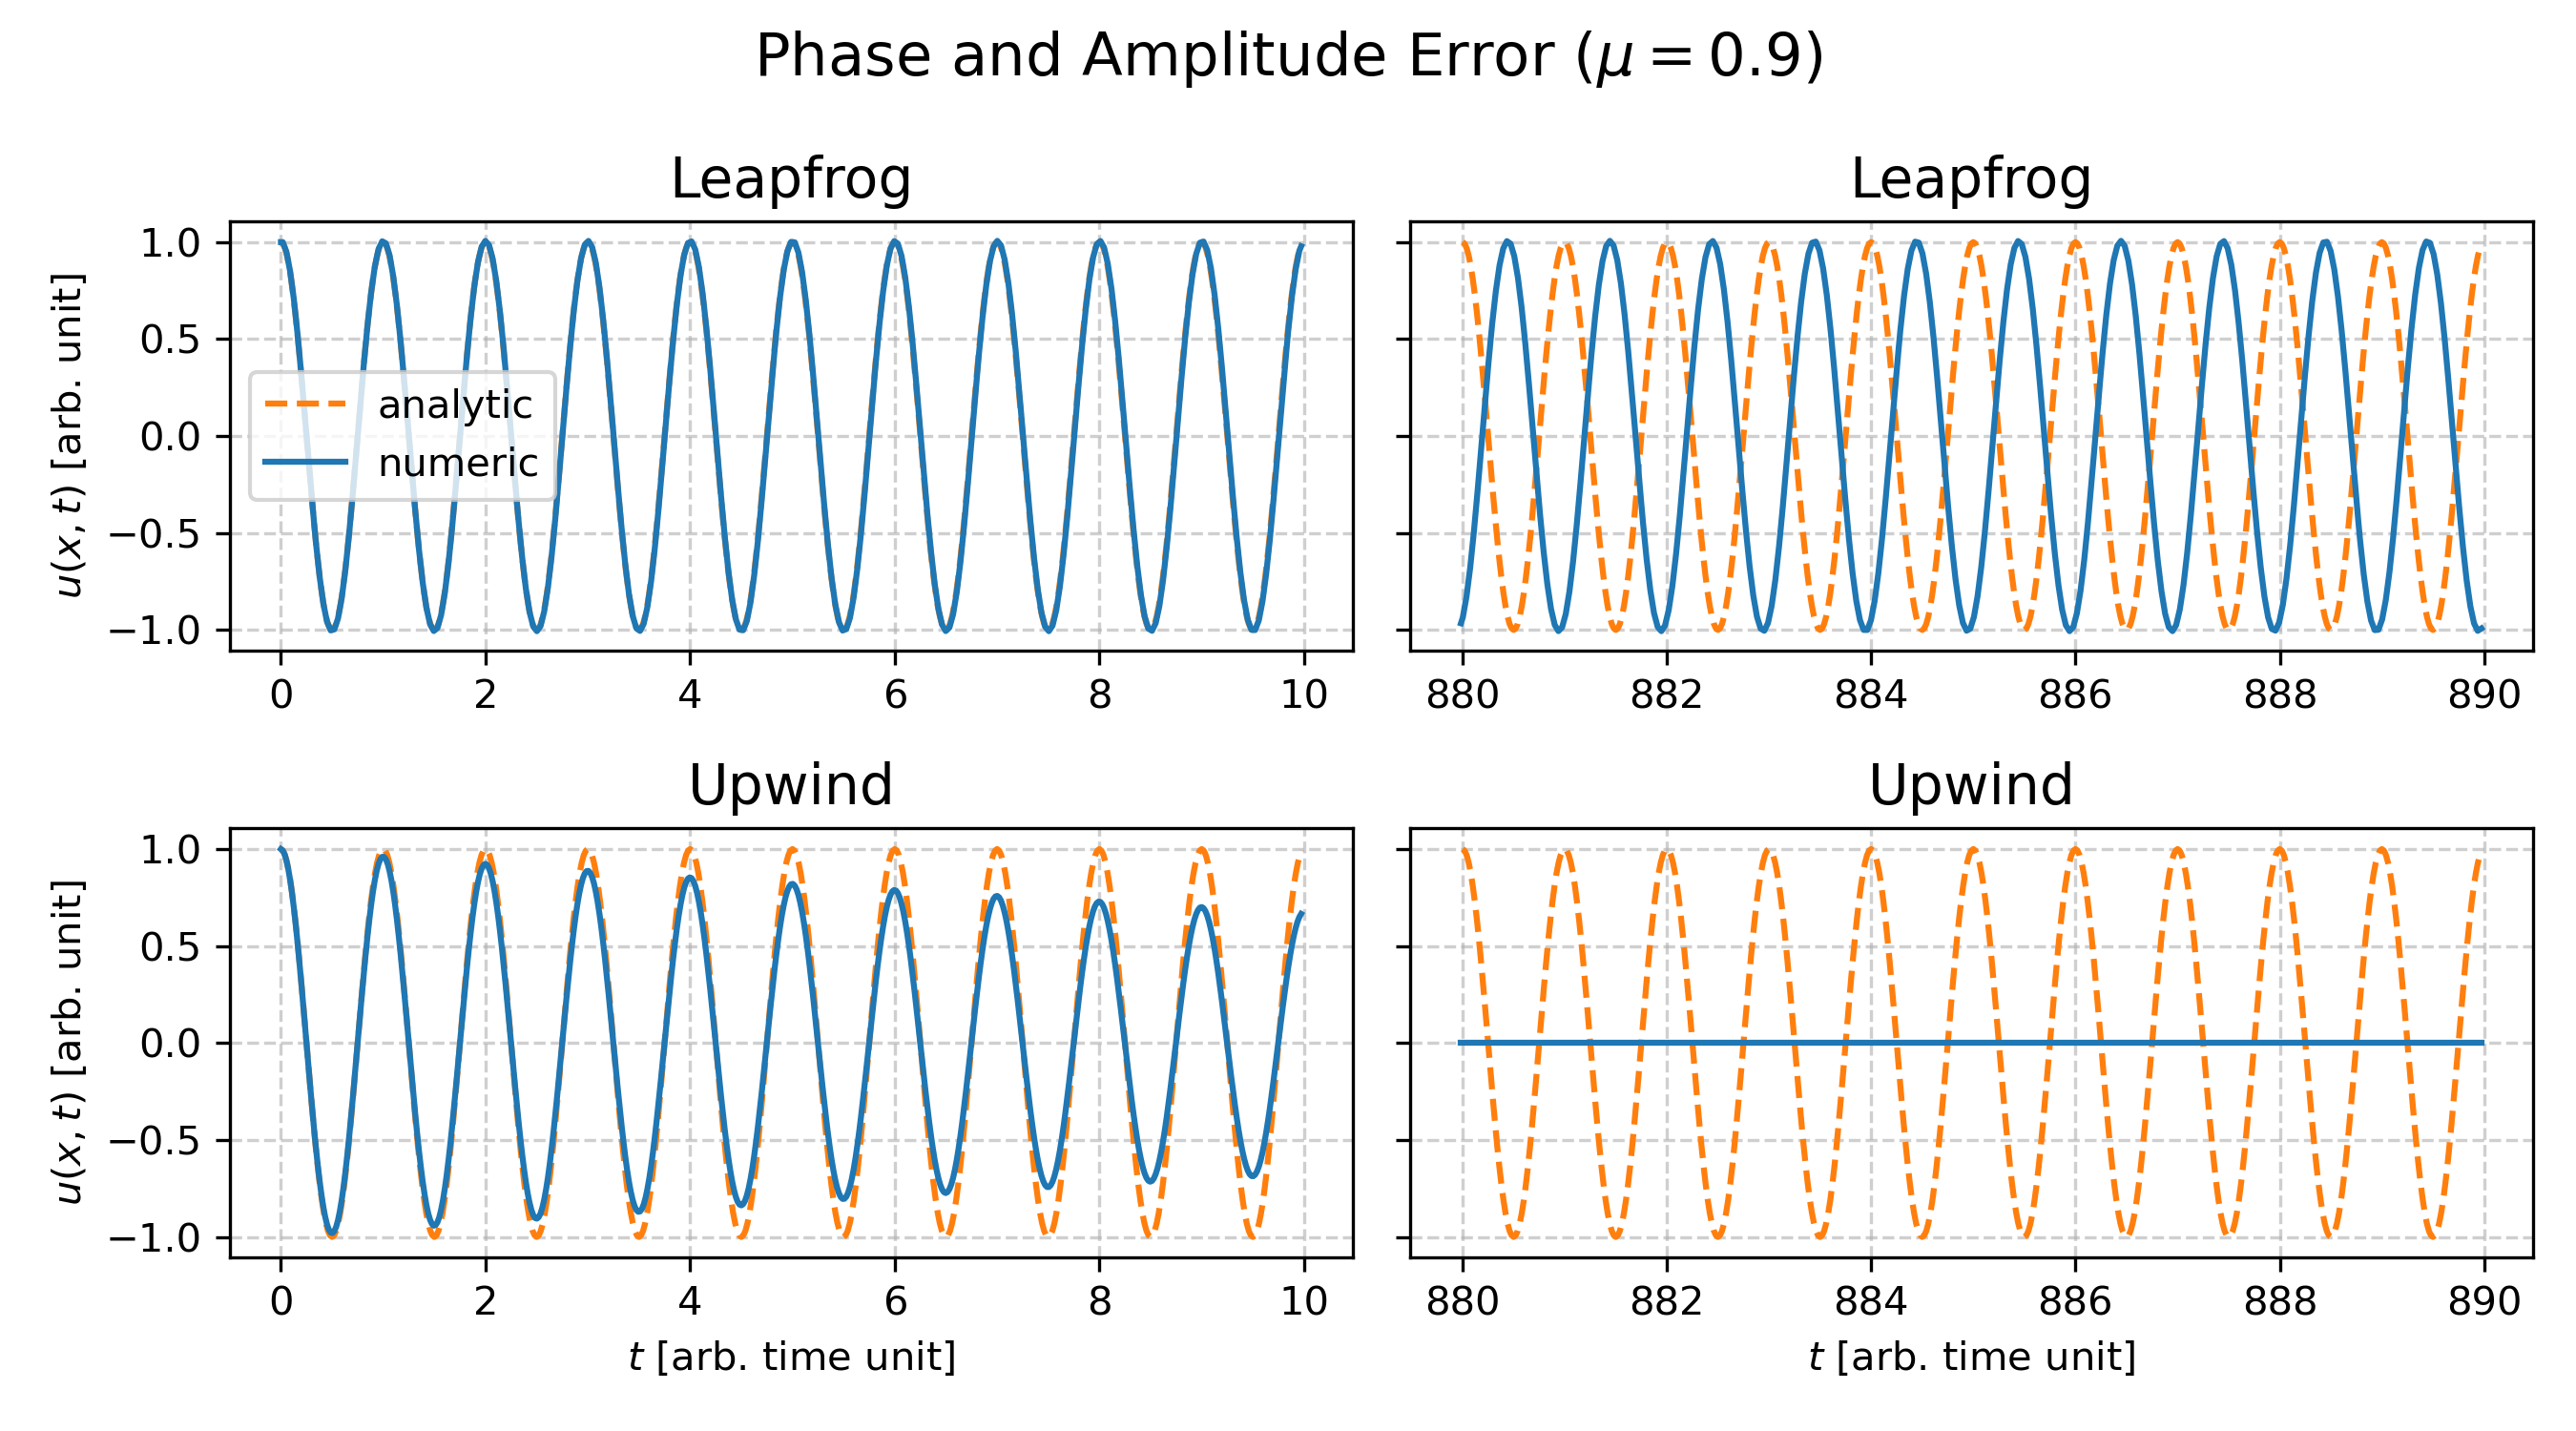
\includegraphics[width=0.8\textwidth]{Figures/phase-errors.png}
    \caption{This figure shows the phase and amplitude errors for the Leapfrog scheme and Upwind scheme.}
    \label{fig:phaseerrors}
\end{figure}

The relative error from the analytic solution can be seen for the different schemes and Courant numbers in \autoref{fig:errors}. There, one can observe that a Courant number of $\mu=1.1$ yielded very large errors after approximately $t \approx 1.0$ arbitrary time units for the Leapfrog scheme and $t \approx 2.5$ arbitrary time units for the Upwind scheme. Furthermore, a Courant number of $\mu=0.9$ for the Upwind scheme did not become unstable, although a non-negligible error arises that grows with time. Both $\mu=0.9$ and $\mu=1.0$ in the Leapfrog scheme show small, but present errors, while $\mu=1.0$ in the Upwind scheme shows very small errors.

\begin{figure}[H]
    \centering
    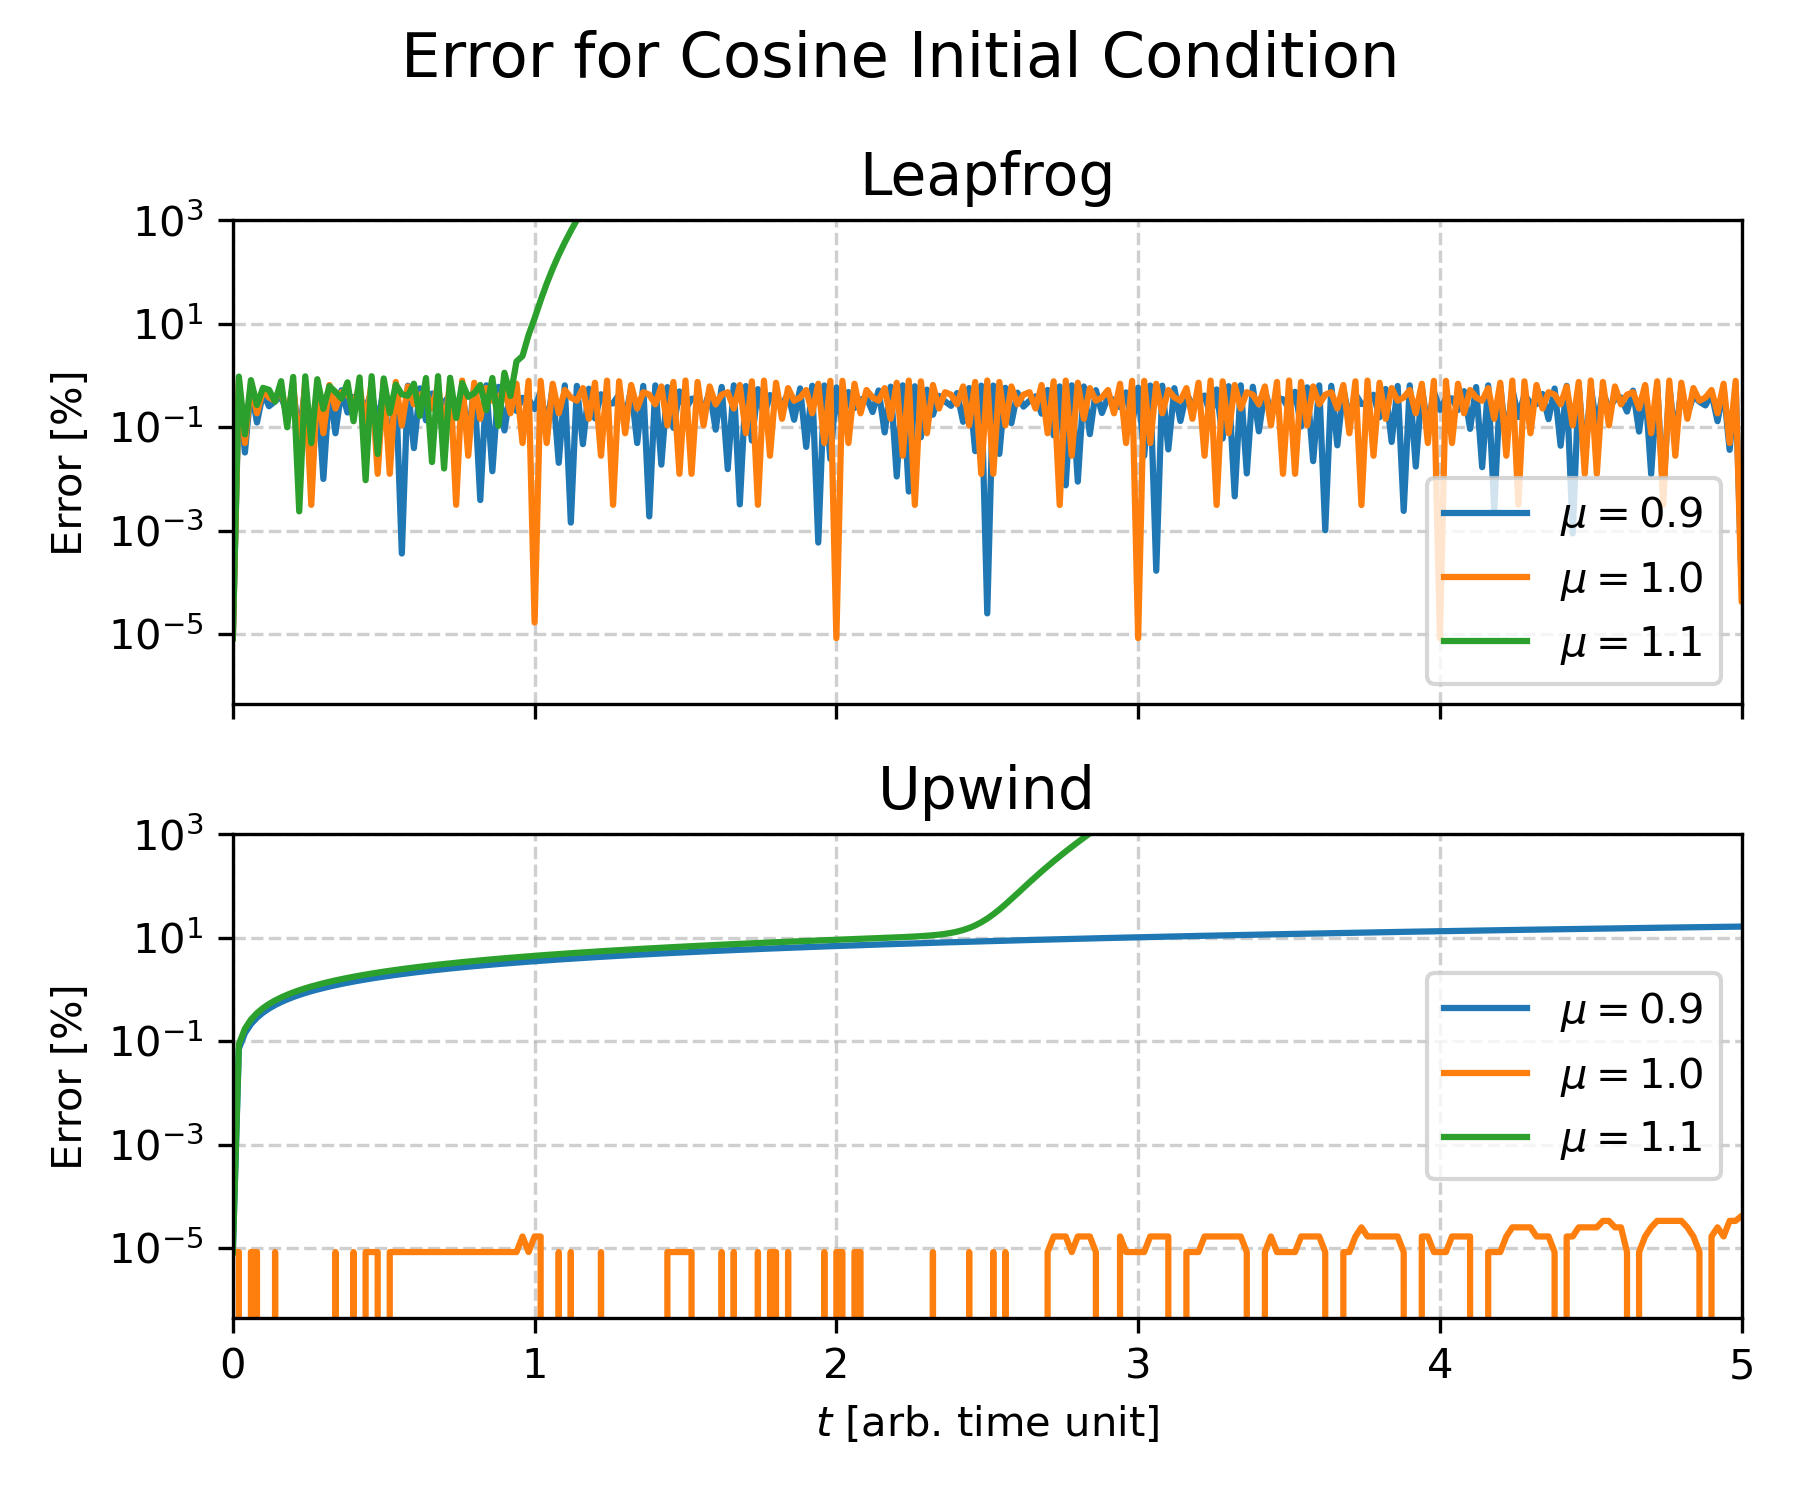
\includegraphics[width=0.55\textwidth]{Figures/errors.png}
    \caption{This figure shows the errors over time, for the different Courant numbers in the Leapfrog scheme and Upwind scheme.}
    \label{fig:errors}
\end{figure}

\subsection{The cosine pulse}

In \autoref{fig:cosinepulse}, one can observe the analytic, Leapfrog, and Upwind results side by side for $\mu=0.9$. Comparing them with the analytic solution, one can observe oscillations after the pulse for the Leapfrog scheme that grow with time. Due to these being oscillations, one can assume this error to originate from the computational mode. In the Upwind scheme, no oscillations can be seen; however, temporal dissipation can be observed.

\begin{figure}[H]
    \centering
    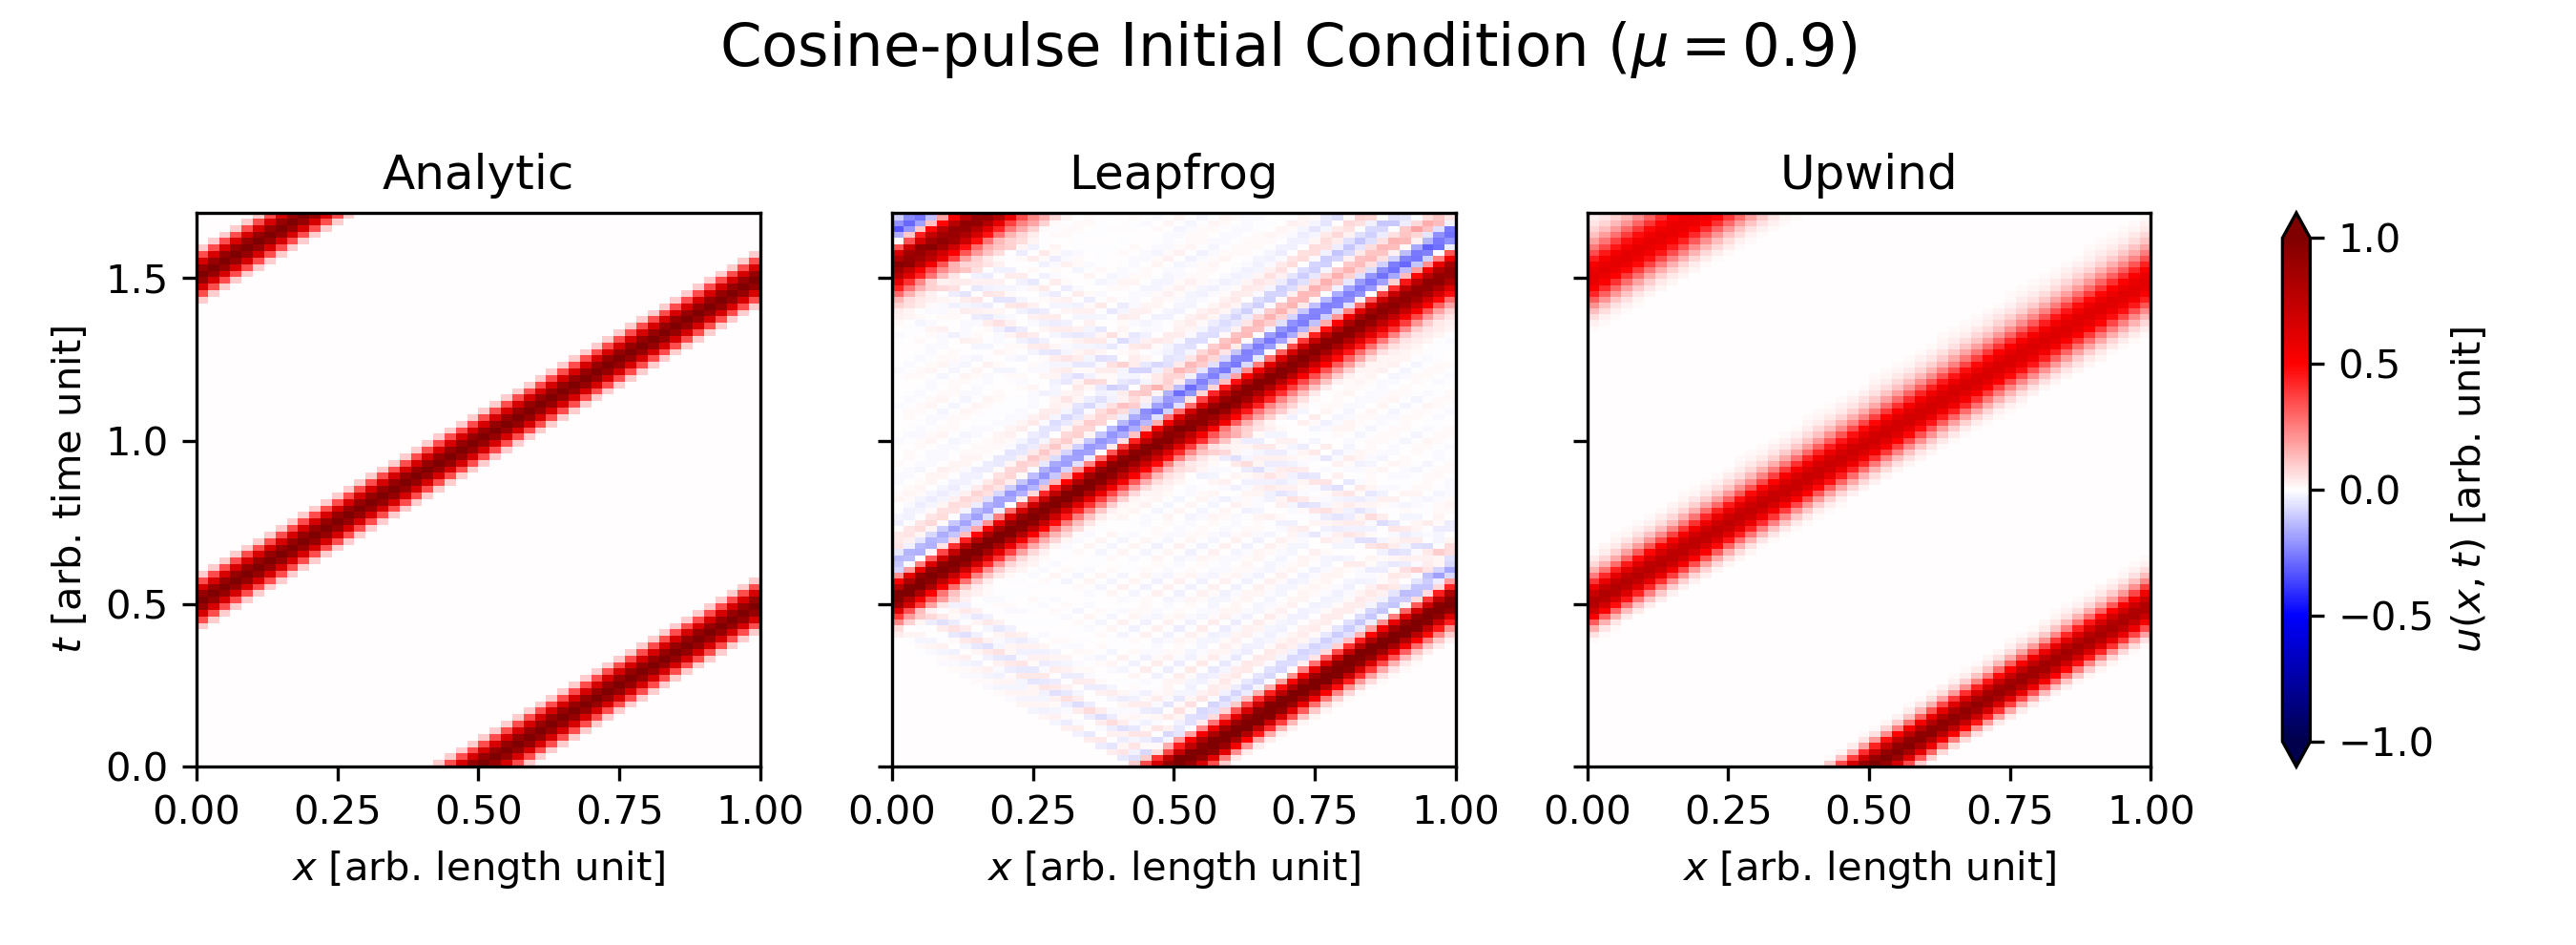
\includegraphics[width=0.95\textwidth]{Figures/cosinepulse-hovmoller.png}
    \caption{This figure shows the solution for the leapfrog scheme, the upwind scheme, along with the analytical solution.}
    \label{fig:cosinepulse}
\end{figure}

In \autoref{fig:cosinepulse-RA}, one can observe what a Robert-Asselin filter, for three different filter parameters, does to the Leapfrog scheme in \autoref{fig:cosinepulse}. One can observe that a filter parameter of $\gamma=0.1$ removed the computational mode oscillations, although an amplitude decrease can be seen. Choosing $\gamma=0.05$ also proved to remove the computational mode without diffusing the data excessively. However choosing $\gamma=0.01$ proved not to remove the computational mode. 

\begin{figure}[H]
    \centering
    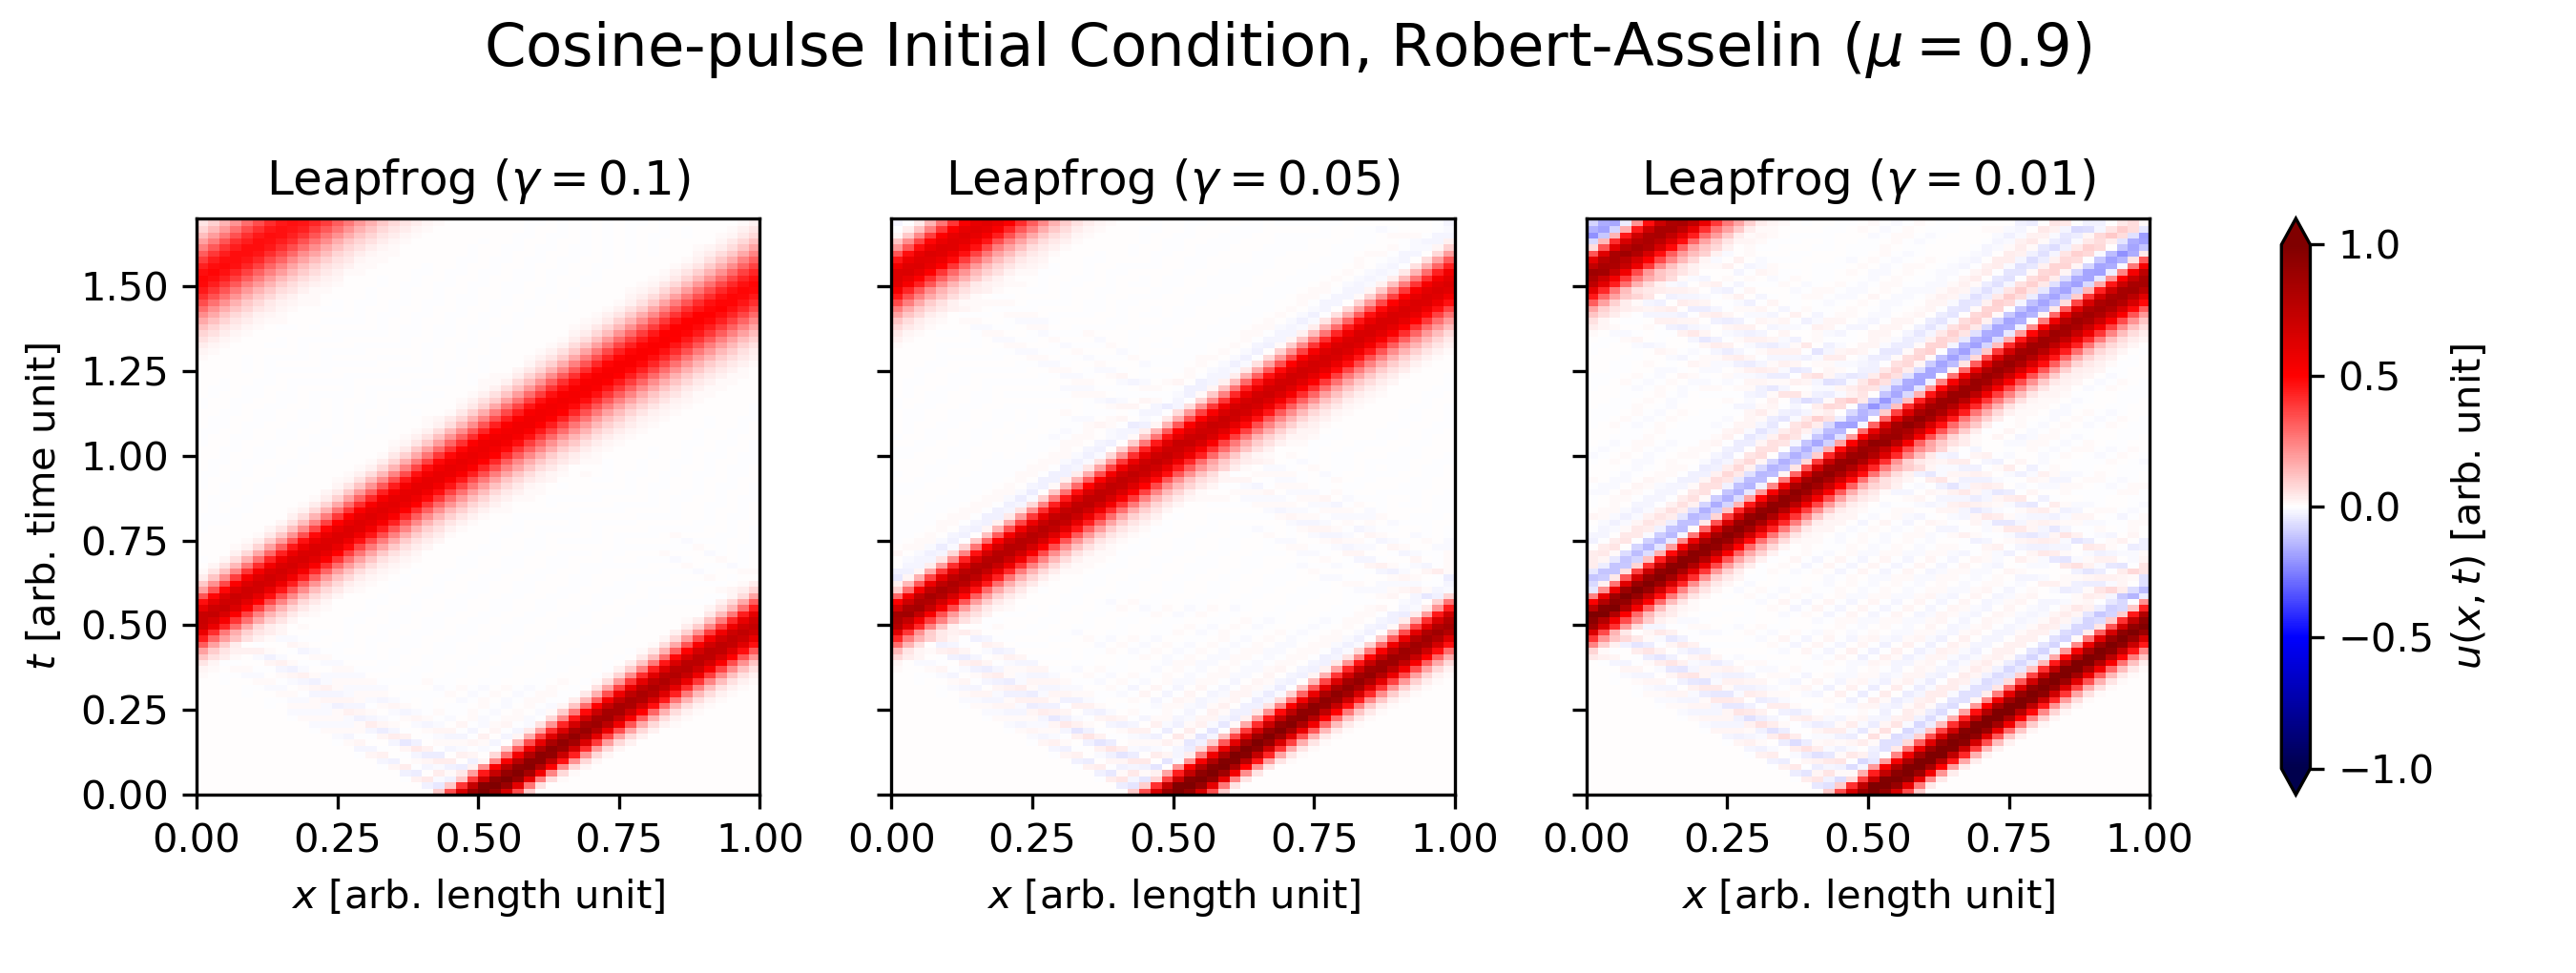
\includegraphics[width=0.95\textwidth]{Figures/cosinepulse-RA-hovmoller.png}
    \caption{This figure shows the effect of the Robert-Asselin filters on the Leapfrog scheme.}
    \label{fig:cosinepulse-RA}
\end{figure}